\documentclass{beamer}
\usepackage{beamerthemesplit}
\usetheme{SPbGU}
%{CambridgeUS}
% Выпишем часть возможных стилей, некоторые из них могут содержать
% дополнительные опции
% Darmstadt, Ilmenau, CambridgeUS, default, Bergen, Madrid, AnnArbor,Pittsburg, Rochester,
% Antiles, Montpellier, Berkley, Berlin
\usepackage{pdfpages}
\usepackage{amsmath}
\usepackage{cmap} % for serchable pdf's
\usepackage[T2A]{fontenc} 
\usepackage[utf8]{inputenc}
\usepackage[english,russian]{babel}
\usepackage{indentfirst}
\usepackage{amsmath}
\usepackage{dot2texi}
\usepackage{tikz}
\usepackage{graphicx}
\usetikzlibrary{shapes,arrows}
\usepackage{fancyvrb}
% Если у вас есть логотип вашей кафедры, факультета или университета, то
% его можно включить в презентацию.

%\usefoottemplate{\vbox{}}%  \tinycolouredline{structure!25}% {\color{white}\textbf{\insertshortauthor\hfill% \insertshortinstitute}}% \tinycolouredline{structure}% {\color{white}\textbf{\insertshorttitle}\hfill}% }}

%\logo{
\includegraphics[width=1cm]{SPbGU_Logo.png}}

%[GLR-анализатор]
\title[]{Cинтаксический анализ динамически формируемых строковых выражений}
%\subtitle[студроект]{Студенческий проект}
\institute[СПбГУ]{
Санкт-Петербургский государственный университет \\
Математико-Механический факультет \\
Кафедра системного программирования }
%[Лукичёв А.С. Григорьев С.В.]


\author[Григорьев Семён]{Григорьев Семён Вячеславович \\
  \and  
  {\bfseries Научный руководитель:} кандидат физико-математических наук, доцент Д.В. Кознов \\ 
%  \and
%  {\bfseries Рецензент:} д.ф.-м.н., проф. Б.К. Мартыненко  
}

\date{2015г.}

\definecolor{orange}{RGB}{179,36,31}

\begin{document}
{

\begin{frame}
\begin{center}
{
\includegraphics[width=1cm]{SPbGU_Logo.png}}
\end{center}
\titlepage
\end{frame}
}

\begin{frame}[fragile]
    \transwipe[direction=90]
    \frametitle{Динамически формируемые строковые выражения: пример}
    \begin{itemize}
        \item Встроенный SQL
\begin{Verbatim}[commandchars=\\\{\}]
\textcolor{blue}{let} p cond fldLst =
    \textcolor{blue}{let mutable} flds = \textcolor{orange}{"id"}
    \textcolor{blue}{for} fld \textcolor{blue}{in} fldLst \textcolor{blue}{do}
        flds <- flds + \textcolor{orange}{", "} + fld 
    \textcolor{blue}{let} tbl = \textcolor{blue}{if} cond \textcolor{blue}{then} \textcolor{orange}{"table1"} \textcolor{blue}{else} \textcolor{orange}{"table2"}    
    \underline{execute} (\textcolor{orange}{"SELECT"} + flds + \textcolor{orange}{"FROM"} + tbl)
\end{Verbatim}
        \item JavaScript в Java
\begin{Verbatim}[commandchars=\\\{\}]
\textcolor{blue}{String} script =
    \textcolor{orange}{"function hello(name) { print(’Hello, ’ + name); }"};
engine.eval(script);
\textcolor{blue}{Invocable} inv = (\textcolor{blue}{Invocable}) engine;
inv.invokeFunction(\textcolor{orange}{"hello"}, \textcolor{orange}{"Scripting!!!"} );
\end{Verbatim}
    \end{itemize}

\end{frame}

\begin{frame}
    \transwipe[direction=90]
    \frametitle{Динамически формируемые строковые выражения: проблемы}
    \begin{itemize}
        \item Значение выражения --- код на некотором языке и его нужно соответствующим образом поддерживать и обрабатывать
        \item Однако для стандартных инструментов это просто строки
        \begin{itemize}
            \item Ошибки в динамически формируемых выражениях обнаруживаются лишь во время выполнения
            \item Нет поддержки в средах разработки
            \item Затруднён реинжиниринг ПО, разработанного с использованием встроенных языков                
        \end{itemize}
        \item Существует множество различных языков и задач
    \end{itemize}
\end{frame}

\begin{frame}
    \transwipe[direction=90]
    \frametitle{Обзор}
    \begin{itemize}
        \item
    \end{itemize}
\end{frame}

\begin{frame}
    \transwipe[direction=90]
    \frametitle{Цели работы}
    \begin{itemize}
        \item Создать подхода к статическому синтаксическому анализу динамически формируемых выражений, позволяющего обрабатывать произвольную регулярную аппроксимацию без потери точности.
        \item Разработать технологию для создания инструментов статического анализа встроенных текстовых языков, реализующей данный алгоритм.
    \end{itemize}
\end{frame}

\begin{frame}
    \transwipe[direction=90]
    \frametitle{Положения, выносимые на защиту}
        \begin{itemize}
            \item Разработан алгоритм синтаксического анализа динамически формируемых выражений, позволяющий обрабатывать произвольную регулярную аппроксимацию множества значений выражения в точке выполнения, реализующий эффективное управление стеком и гарантирующий конечность представления леса вывода. Доказана завершаемость и корректность предложенного алгоритма.
            \item Создана архитектура инструментария для разработки программных средств синтаксического анализа динамически формируемых строковых выражений.
            \item Разработана методика анализа динамически формируемых строковых выражений в проектах по реинжинирингу информационных систем.  
        \end{itemize}
\end{frame}

\begin{frame}
    \transwipe[direction=90]
    \frametitle{Научная новизна}
    \begin{itemize}
        \item Предложенный алгоритм предназначен для синтаксического анализа динамически формируемых выражений и построения компактной структуры данных, содержащей для всех корректных значений выражения их деревья вывода.
        \item Предложена архитектура инструментального средства, позволяющего упростить создание новых инструментов для анализа динамически формируемых выражений на любых языках программирования.
    \end{itemize}
\end{frame}

\begin{frame}
    \transwipe[direction=90]
    \frametitle{Архитектура: постановка задачи}
\end{frame}

\begin{frame}
    \transwipe[direction=90]
    \frametitle{Архитектура: процесс анализа}
    \begin{center}
        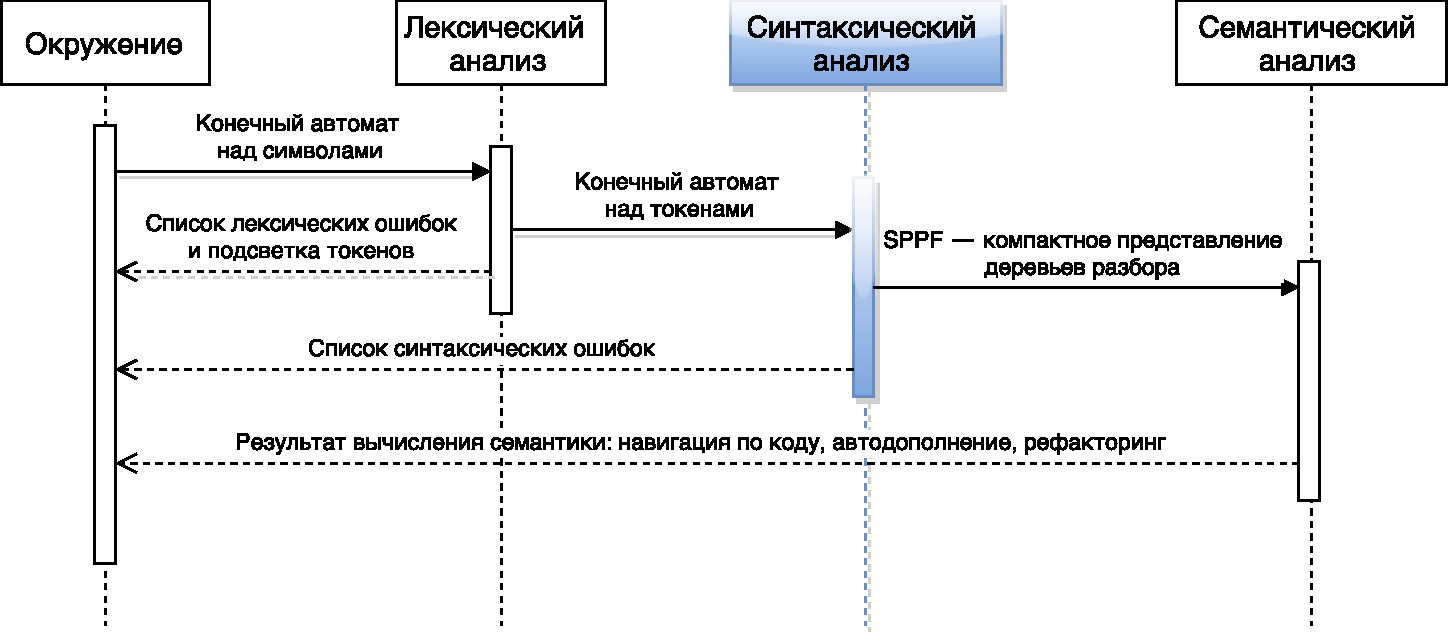
\includegraphics[width=300pt]{pictures/Seq.pdf}
    \end{center}
\end{frame}

\begin{frame}
    \transwipe[direction=90]
    \frametitle{Архитектура: инструментарий}
    \begin{center}
        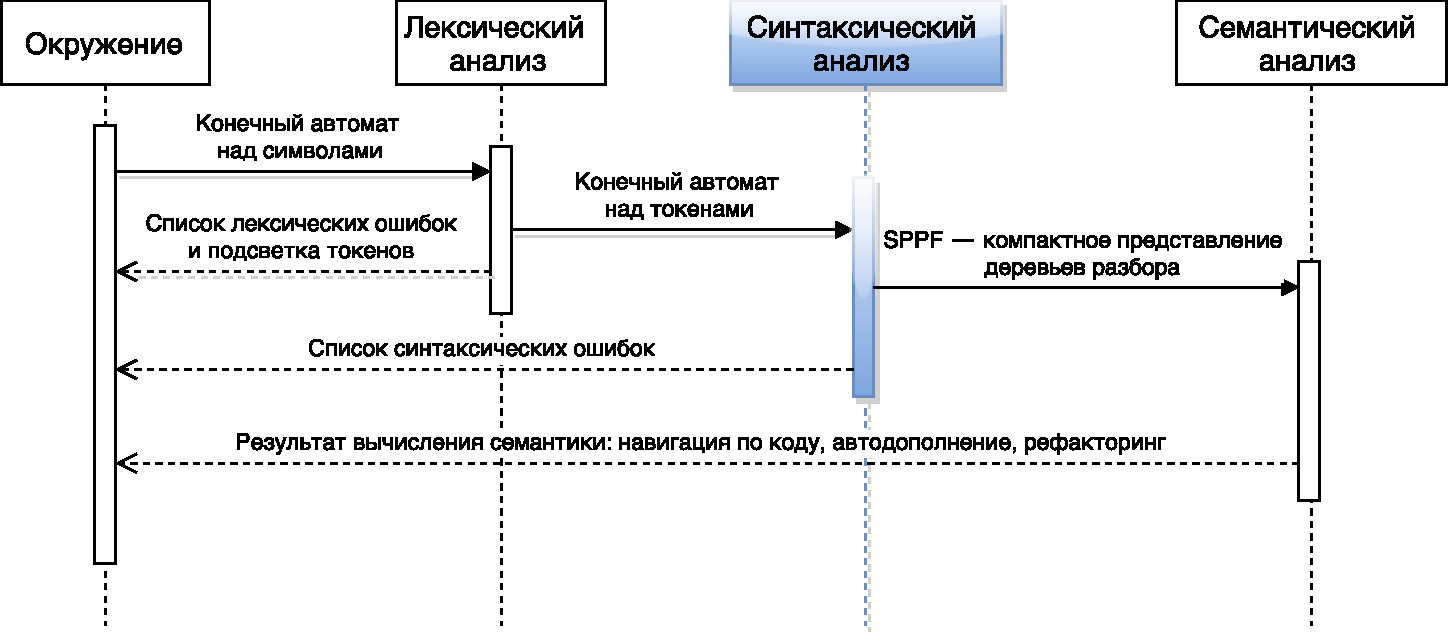
\includegraphics[width=300pt]{pictures/Seq.pdf}
    \end{center}
\end{frame}

\begin{frame}
    \transwipe[direction=90]
    \frametitle{Архитектура: аппроксимация и лексический анализ}    
\end{frame}

\begin{frame}
    \transwipe[direction=90]
    \frametitle{Алгоритм: постановка задачи}
\end{frame}

\begin{frame}
    \transwipe[direction=90]
    \frametitle{Алгоритм: описание}
\end{frame}

\begin{frame}
    \transwipe[direction=90]
    \frametitle{Алгоритм: завершаемость}
    \begin{theorem}


    \end{theorem}

    \begin{proof}


    \end{proof}

\end{frame}

\begin{frame}
    \transwipe[direction=90]
    \frametitle{Алгоритм: корректность}
    \begin{theorem}

    \end{theorem}

    \begin{proof}


    \end{proof}


    \begin{theorem}

    \end{theorem}

    \begin{proof}


    \end{proof}


\end{frame}

\begin{frame}
    \transwipe[direction=90]
    \frametitle{Алгоритм: пример работы}
\end{frame}

\begin{frame}[t]
    \transwipe[direction=90]
    \frametitle{Методология}
    \begin{itemize}
        \item
    \end{itemize}
\end{frame}

\begin{frame}[t]
    \transwipe[direction=90]
    \frametitle{Апробация: синтетические замеры}
\end{frame}

\begin{frame}[t]
    \transwipe[direction=90]
    \frametitle{Апробация: трансляция динамического SQL}
\end{frame}

\begin{frame}[t]
    \transwipe[direction=90]
    \frametitle{Апробация: плагин к ReSharper}
\end{frame}

\begin{frame}
    \transwipe[direction=90]
    \frametitle{Публикации}
  \begin{itemize}
      \item Кириленко Я.А., Григорьев С. В., Авдюхин Д. А. Разработка синтаксических анализаторов в проектах по автоматизированному реинжинирингу информационных систем.  Научно-технические ведомости Санкт-Петербургского государственного политехнического университета информатика, телекоммуникации, управление. Т. 3, N 174, 2013. C. 94 --- 98.
      \item Григорьев С. В., Вербицкая Е. А., Полубелова М. И., Иванов А. В., Мавчун Е. В. Инструментальная поддержка встроенных языков в интегрированных средах разработки. Моделирование и анализ информационных систем. Т. 21, N 6, 2014. С. 131---143.
          \item Григорьев С.В. Алгоритм синтаксического анализа динамически формируемых выражений.
  \end{itemize} 
\end{frame}

\begin{frame}
    \transwipe[direction=90]
    \frametitle{Публикации}
  \begin{itemize}
          \item Semen Grigorev, Iakov Kirilenko. GLR-based abstract parsing. In Proceedings of the 9th Central \& Eastern European Software Engineering Conference in Russia (CEE-SECR ’13). 2013. ACM, New York, NY, USA. 1-9 p.
          \item Semen Grigorev, Ekaterina Verbitskaia, Andrei Ivanov, Marina Polubelova, Ekaterina Mavchun. String-embedded language support in integrated development environment. In Proceedings of the 10th Central and Eastern European Software Engineering Conference in Russia (CEE-SECR '14). 2014. ACM, New York, NY, USA. 1-11 p.
          \item Semen Grigorev, Iakov Kirilenko. From Abstract Parsing to Abstract Translation. Proceedings of the Spring/Summer Young Researchers' Colloquium on Software Engineering. 2014. Saint Petersburg, Russia. 1-5 p.
  \end{itemize} 
\end{frame}

\end{document}
